\section{Day 10: Metric Spaces (Oct. 3, 2024)}
Outfit of the day! jungle story / africa circles shirt
\begin{figure}[h]
    \centering
    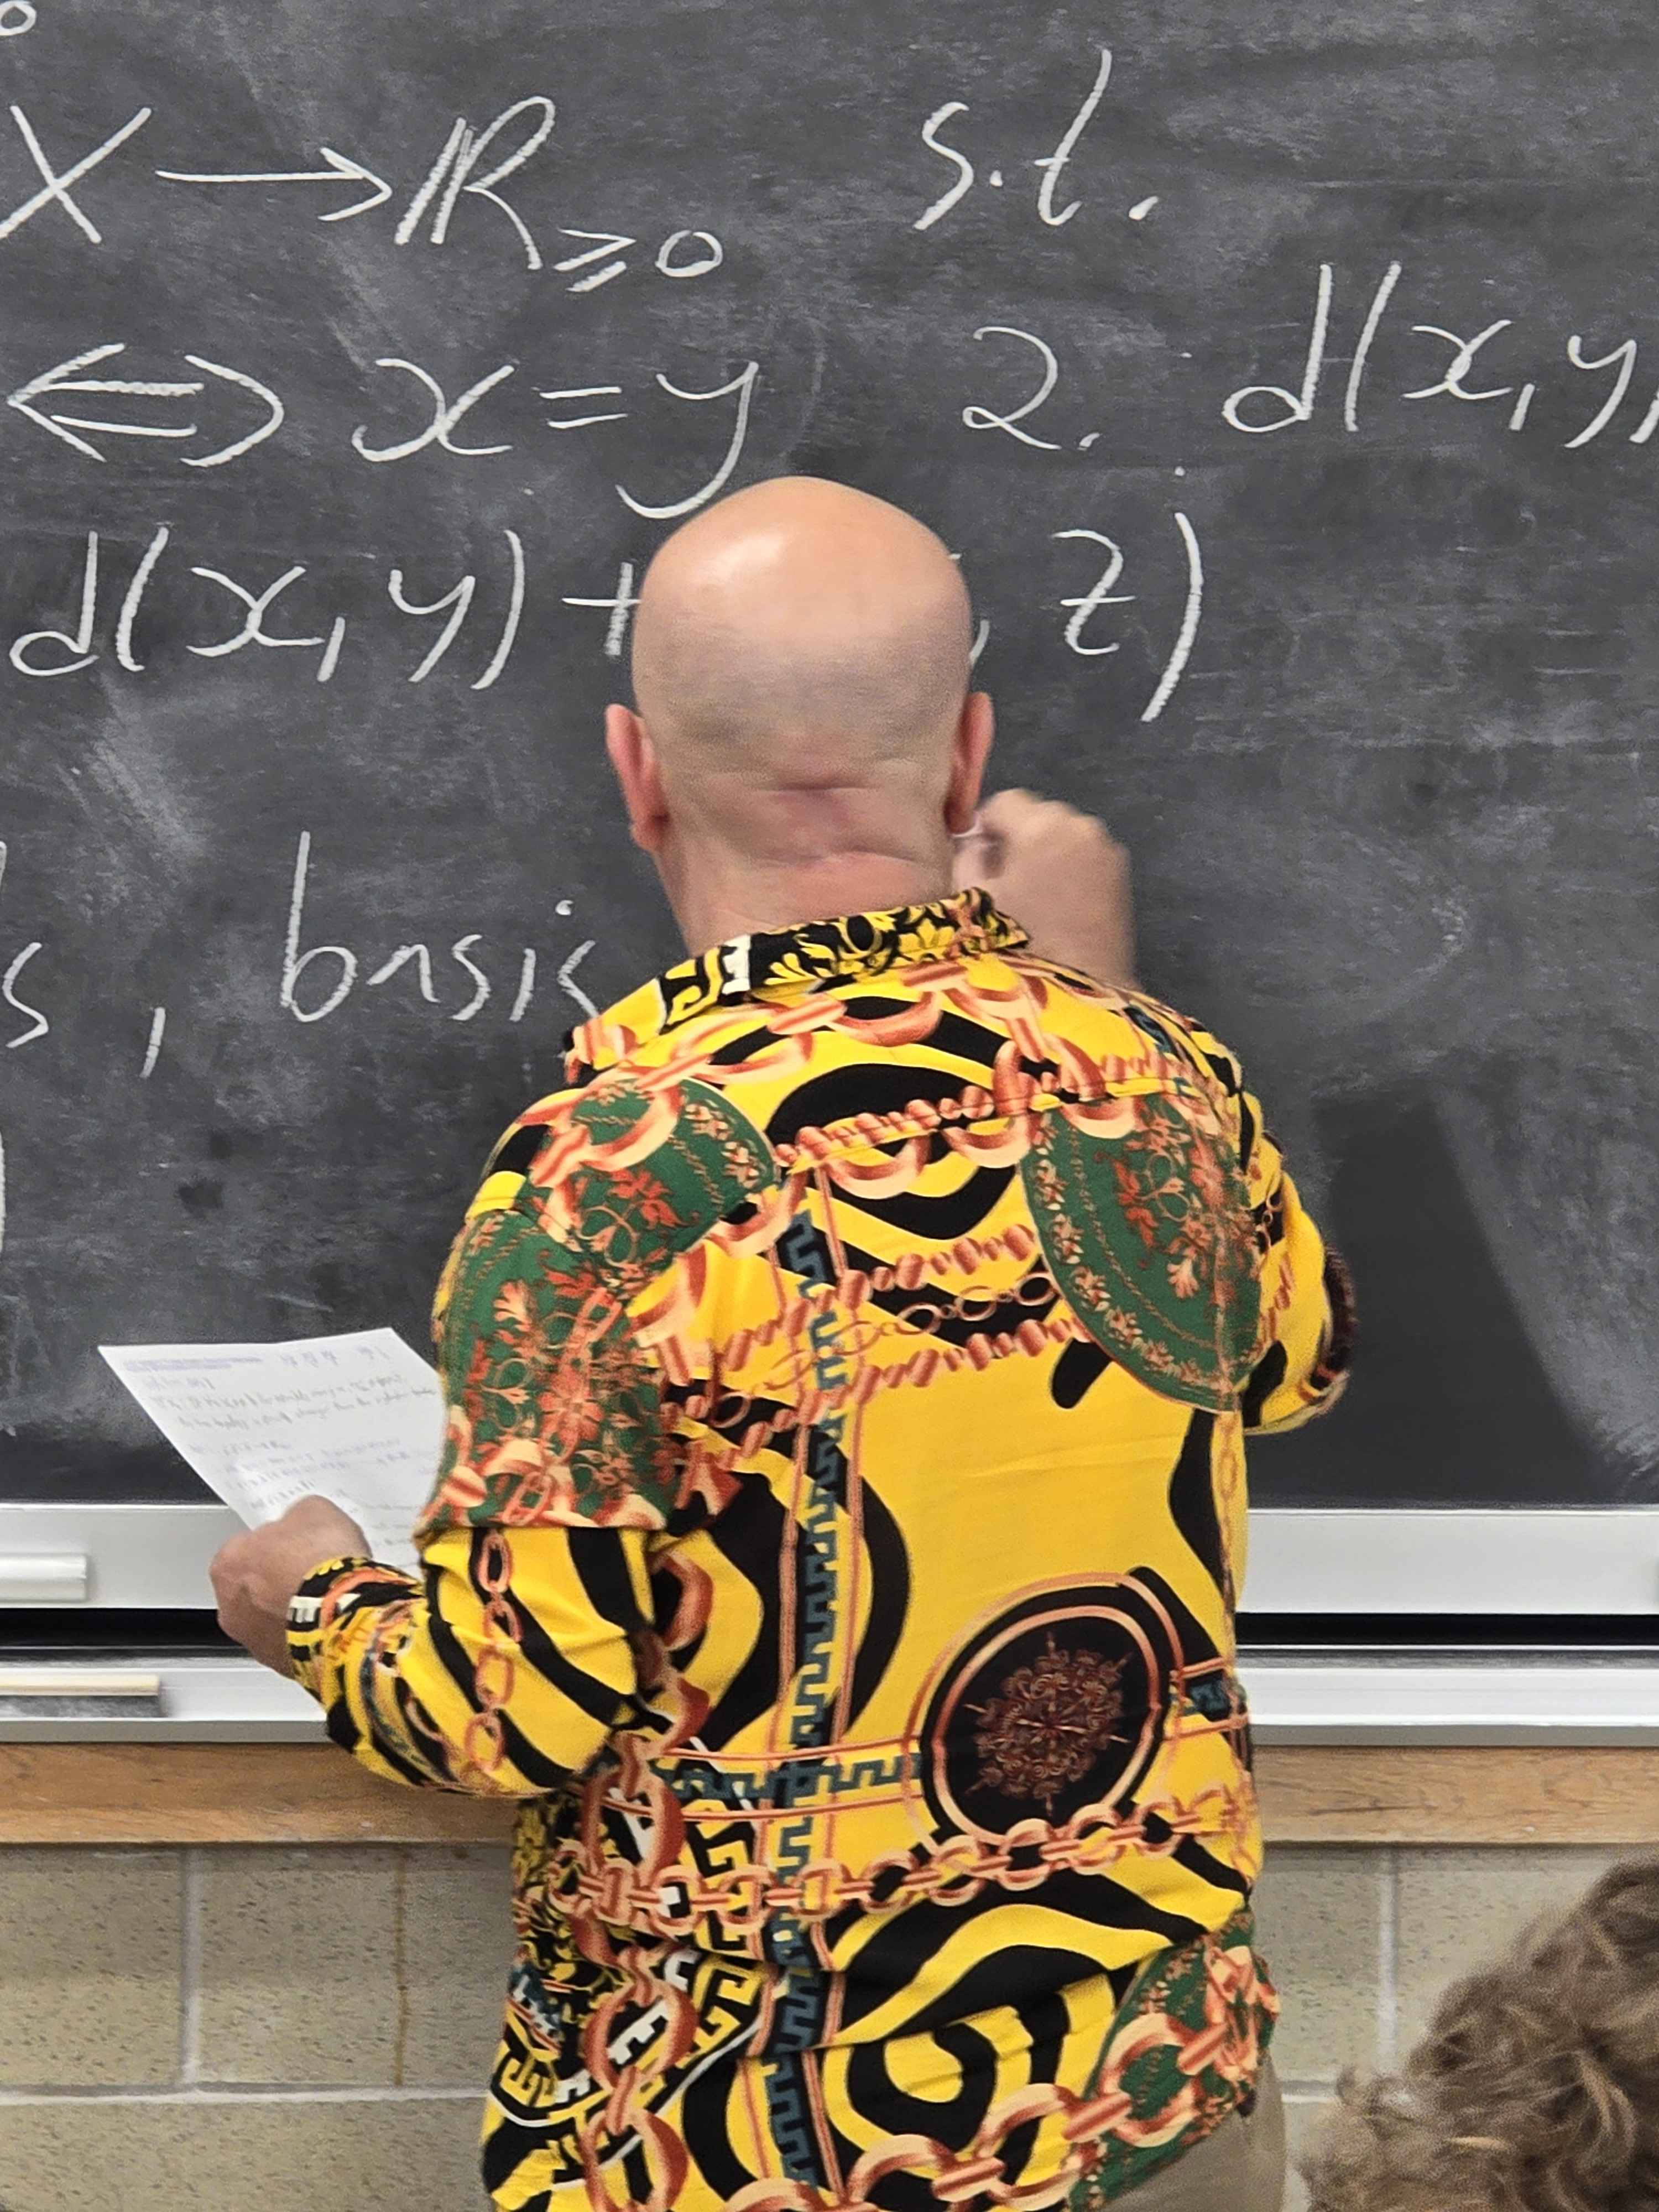
\includegraphics[scale=0.1]{MAT327 Notes/Dror Shirts/dror day 10 shirt.jpg}
\end{figure}

Recap: let $d : X \times X \to \RR_{\geq 0}$ be a metric. Then $d$ is defined to have the properties,
\begin{enumerate}[label=(\alph*)]
    \item $d(x, y) = 0$ if and only if $x = y$;
    \item $d(x, y) = d(y, x)$;
    \item $d(x, z) \leq d(x, y) + d(y, z)$.
\end{enumerate}
In particular, the balls $B_r(x)$ forming a basis on the metric topologoy means that such spaces are always $T_2$.
\medskip\newline
Let us consider $\prod X_\alpha$, and consider $H_\alpha \subset X_\alpha$ for all indices $\alpha$ to be open, nonempty, and non-full (not $X_\alpha$). Then $\prod H_\alpha$ is open in the box topology, but it contains not even one cylinder. So the box topology is strictly stronger than the cylinder topology, except if there exists $\alpha$ such that some $X_\alpha = \emptyset$ and not too many of them have the trivial topology.\footnote{wtf? time for me to read more munkres}

\newpage
\noindent A topological space $X$ is called ``metrizable'' if there is a metric $d$ on $X$ that induces its topology. Note that $d$ is far from unique. We now consider some examples:
\begin{enumerate}[label=(\alph*)]
    \item $\RR^\NN_\mathrm{box}$ is not metrizable.
    \item $\RR^\RR_\mathrm{cyl}$ is also not metrizable (read: set of functions $f : \RR to \RR$).
\end{enumerate}
Recall that in a topological space, $x_n$ converges to $x$ (i.e., $x_n \to x$) if every neighborhood of $x$ contains almost all of the $x_n$'s (read: an infinite amount or except for finitely many $x_n$'s). A similar definition holds in metric spaces; however, here, it is enough to look at the balls $B_\eps(x)$ for all $\eps > 0$. We may write this as
\[ \forall \eps > 0, \exists N \, s.t. \,\, n > N \implies \left(x_n \in B_\eps(x) \iff d(x_n, x) < \eps\right). \]
Thus, $d(x_n, x) \xrightarrow[]{n \to \infty} 0$.
\medskip\newline
Given a topological space $X$ with $A \subset X$, then the sequential closure of $A$ in $X$, i.e. $\mathrm{scl}_X(A) = \{x \in X \mid \exists x_1, x_2, \dots \, s.t. \,\, x_n \to x\}$.\footnote{note that in class, dror uses seq-cl instead of scl for sequential closure. i just can't get it to work on latex :<}

\begin{simpleclaim}[Sequential Closure is in Closure]
    We claim that $\mathrm{scl}\,(A) \subset \mathrm{cl}\,(A)$.
\end{simpleclaim}
\noindent For any $x$ in the sequential closure of $A$ such that $x_n \to x$, every neighborhood of $x$ contains almost all of the $x_n$'s, so it intersects $A$. Thus, $x \in \mathrm{cl}\,(A)$. \qed

\begin{simpleclaim}[Equality of Sequential Closure and Closure in Metrizable $X$]
    If $X$ is metrizable, and $A \subset X$, then $\mathrm{cl} (A) = \mathrm{scl} (A)$.
\end{simpleclaim}
\noindent Pick any metric $d$ that induces the topology of $X$. For any $n \geq 1$, $B_{d, \frac{1}{n}}(x)$ (new notation! read: the ball of radius $\frac{1}{n}$ about $x$ w.r.t. the metric $d$) is an open neighborhood of $x$, and so $B_{d, \frac{1}{n}}(x) \cap A \neq \emptyset$. So choose $x_n \in B_{d, \frac{1}{n}}(x) \cap A$, meaning $x_n \to x$. Indeed, if $U$ is a neighborhood of $x$, so $U$ contains some ball of radius $\eps$ which contains $x$. Namely, there exists $y \in X$ and there exists $\eps > 0$ such that $x \in B_\eps(y) \subset U$.
\medskip\newline
Take $\delta = \eps - d(x, y)$, and now $x \in B_\delta(x) \subset B_\eps(y) \subset U$. If $n > \frac{1}{\delta}$, then $\frac{1}{n} < \delta$, so $x_n \in B_{\frac{1}{n}}(x) \subset B_\delta(x) \subset U$. Thus, the sequence $x_n$ indeed converges to the point $x$. \qed
\medskip\newline
\noindent We now return to prove examples (a) and (b).
\begin{enumerate}[label=(\alph*)]
    \item We will prove this by considering both directions. Let $X = \RR^\NN_\mathrm{box}$, $A = \RR^\NN_{>0}$, i.e. $A$ is the set of sequences of positive numbers. Let $x = \overline{0} = (0, 0, 0, \dots)$. Clearly, $\overline{0}$ is in the closure of $A$. Indeed, if $\prod (a_i, b_i)$ is a basic neighborhood of $\overline{0}$, i.e. $a_i < 0 < b_i$, then the sequence $\left(\frac{b_i}{2}\right)_{i=1}^\infty \in U \cap A$, and so $U \cap A \neq \emptyset$.
    \medskip\newline
    For the harder side, we claim that $\overline{0} \not\in \mathrm{scl}\,(A)$. For contradictoin, suppose that $\overline{0}$ is in the sequential closure, i.e. $x_i \in A$ such that $x_i \to \overline{0}$ (read: each $x_i$ itself is a sequence). Namely, $x_i = (x_{ij})_{j \in \NN}$, where $x_{ij} > 0$ for all $i, j$. Let $U = \prod (a_i, b_i)$. We may take $a_i = -327$ (random negative number). We may then take $b_1 = \frac{x_{11}}{2}$, $b_2 = \frac{x_{22}}{2}$, etc... with $b_i = \frac{x_{ii}}{2}$. Thus, we have
    \[ U = \prod_{i=1}^\infty \left(-327, \frac{x_{ii}}{2}\right). \]
    Then $\overline{0} \in U$, yet for all $i$, $x_i \not\in U$ as $x_{ii} \geq \frac{x_{ii}}{2}$. So it is not true that almost all of the $x_i$'s belong to $U$. \qed

    \newpage
    \item Let $X = \RR_\mathrm{cyl}^\RR$. Let
    \begin{align*}
        B := \{\text{beds of nails}\} &= \{f : \RR \to \RR \mid f = 0 \text{ except on finitely many } x\} \\
        &= \{ f \mid \exists \text{ finite } A_f \subset \RR \, s.t. \,\, f(x) = 0 \text{ if } x \not\in A_f \}.
    \end{align*}
    Then $\mathrm{cl}\,(B) = X$. The sequential closure $\mathrm{scl}\,(B)$ is given as an exercise. Indeed, for example, the function $e^x \in \mathrm{cl}\,(B)$, even if $e^x$ is clearly not a bed of nails. Suppose $U$ is a neighborhood of $e^x$. $U$ is defined by constraining finitely many coordinates $x \in \RR$ in open intervals $(a_x, b_x)$ (read: on the $y$-axis) for each given $x$. Then there is a bed of nails satisfying these constraints.
    \begin{simpleclaim}
        We claim that the constant function, $\overline{1}(x) = 1$, does not belong in the sequential closure of beds of nails.
    \end{simpleclaim}
    Suppose $f_n \in B$ (a sequence of $f_1, f_2, \dots$ where we sequentially add more and more nails with each $f_i$), and $f_n \xrightarrow[]{\mathrm{cyl}} \overline{1}$. Then let $A_n = \sup (f_n) = \{ x \mid f_n(x) \neq 0 \}$ be a finite set. $\bigcup A_n$ is countable, hence $\bigcup A_n \subsetneq \RR$. Thus, we may pick $y \not\in \bigcup A_n$, meaning $f_n(y) = 0$ for every $n$.
    \medskip\newline
    Pick a neighborhood of $\overline{1}$, $U = \{f \mid f(y) > 0 \}$. Then $U$ is open in the cylinder topology because we've only constrained $1$ coordinate to be in the open set. Thus, $\overline{1} \in U$ and for all $n$, $f_n \in U$, and so $f_n \not\to \overline{1}$.
\end{enumerate}

\begin{simplethm}[Countable Product of Metrizable Spaces]
    The countable product of metrizable spaces is also metrizable in the cylinder topology, i.e., if $X_n$ is metrizable for all $n$, then $\left(\prod_{n=1}^\infty X_n\right)_\mathrm{cyl}$ is metrizable.
\end{simplethm}
\noindent Given $(X_n, d_n)$, we need a metric on $\prod X_n = \{(x_n) \mid x_n \in X_n\}$. Then $d\left((x_n), (y_n)\right) = \sup\left( \frac{\overline{d_n}(x_n, y_n)}{n} \right)$.
\begin{simplelemma}
    If $d$ is a metric, then so is $\overline{d}(x, y) = \min\{1, d(x, y)\}$, and it induces the same topology as $d$.
\end{simplelemma}
\noindent We start by noting that $\overline{d}$ is a metric.
% https://q.uiver.app/#q=WzAsMyxbMCwxLCIoeCkiXSxbMiwxLCIoeikiXSxbMSwwLCIoeSkiXSxbMCwxLCJkXzMgPSBkKHgseikiLDIseyJzdHlsZSI6eyJoZWFkIjp7Im5hbWUiOiJub25lIn19fV0sWzIsMSwiZF8yID0gZCh5LHopIiwwLHsibGFiZWxfcG9zaXRpb24iOjkwLCJzdHlsZSI6eyJoZWFkIjp7Im5hbWUiOiJub25lIn19fV0sWzIsMCwiZF8xID0gZCh4LHkpIiwyLHsibGFiZWxfcG9zaXRpb24iOjkwLCJzdHlsZSI6eyJoZWFkIjp7Im5hbWUiOiJub25lIn19fV1d
\[\begin{tikzcd}
	& {(y)} \\
	{(x)} && {(z)}
	\arrow["{d_1 = d(x,y)}"'{pos=0.9}, no head, from=1-2, to=2-1]
	\arrow["{d_2 = d(y,z)}"{pos=0.9}, no head, from=1-2, to=2-3]
	\arrow["{d_3 = d(x,z)}"', no head, from=2-1, to=2-3]
\end{tikzcd}\]
If $d_1 + d_2 \leq 1$, then $d_3 \leq 1$ and now $\overline{d_i} = d_i$. If $d_1 + d_2 > 1$, then $\overline{d_1} + \overline{d_2} \geq 1 \geq \overline{d_3}$. Now, let $\SB = \{B_r(x)\}$ be replaced with the set $\{B_r(x) \mid r < \frac{1}{7}\}$ or some arbitrary constant less than $1$ (for now, we pick $\frac{1}{7}$). Then $d, \overline{d}$ induce the same topology because their small balls are the same. \qed
\medskip\newline
\noindent We now claim that if $(X_n, d_n)$ are metric spaces, then defining $d((x_n), (y_n)) = \sup_n \overline{d_n}(x_n, y_n)$ is a metric on $X = \prod X_n$ called ``the uniform metric on $X$''. It defines neither the box nor the cylinder topology.
\medskip\newline
\noindent We will continue the proof next lecture.